\documentclass[12pt,a4paper]{article}
\usepackage{algorithm, algpseudocode, amsmath, amssymb, caption, csquotes, empheq, geometry, graphicx, hyperref, listings, multirow, physics, siunitx, subcaption, upgreek}
\usepackage[section]{placeins}

\title{Computational Physics\\Problem Set 3}
\author{Saleh Shamloo Ahmadi\\Student Number: 98100872}
\date{October 18, 2021}

\hypersetup{colorlinks=true, urlcolor=cyan}
\newcommand{\percfig}{../fig/percolation}
\newcommand{\rwfig}{../fig/random-walk}

\begin{document}
	\maketitle
	\section{Percolation}
	Note: we simulate \emph{site percolation}.
	\subsection{Correlation Length}
	The correlation length $\xi$ is a measure of the radius of the maximum closed (non-infinite) cluster;
	This shows the maximum length of interactions before phase transition occures and the lattice either becomes
	homogenous or clusters are broken off.
	
	In our analysis, we use the maximum radius of gyration of closed clusters to measure the correlation length
	(any similar measure is valid).

	The correlation length diverges (or peaks, for a finite lattice) at the critical probability $p_c$ of forming sites
	in the lattice; This is because at higher probabilities, percolation happens frequently and there are less clusters
	and at lower probabilites, clusters break off more at smaller length scales.
	
	\newgeometry{left=0in, right=0in}
	\begin{figure}
		\centering
		\begin{subfigure}{0.45\linewidth}
			\centering
			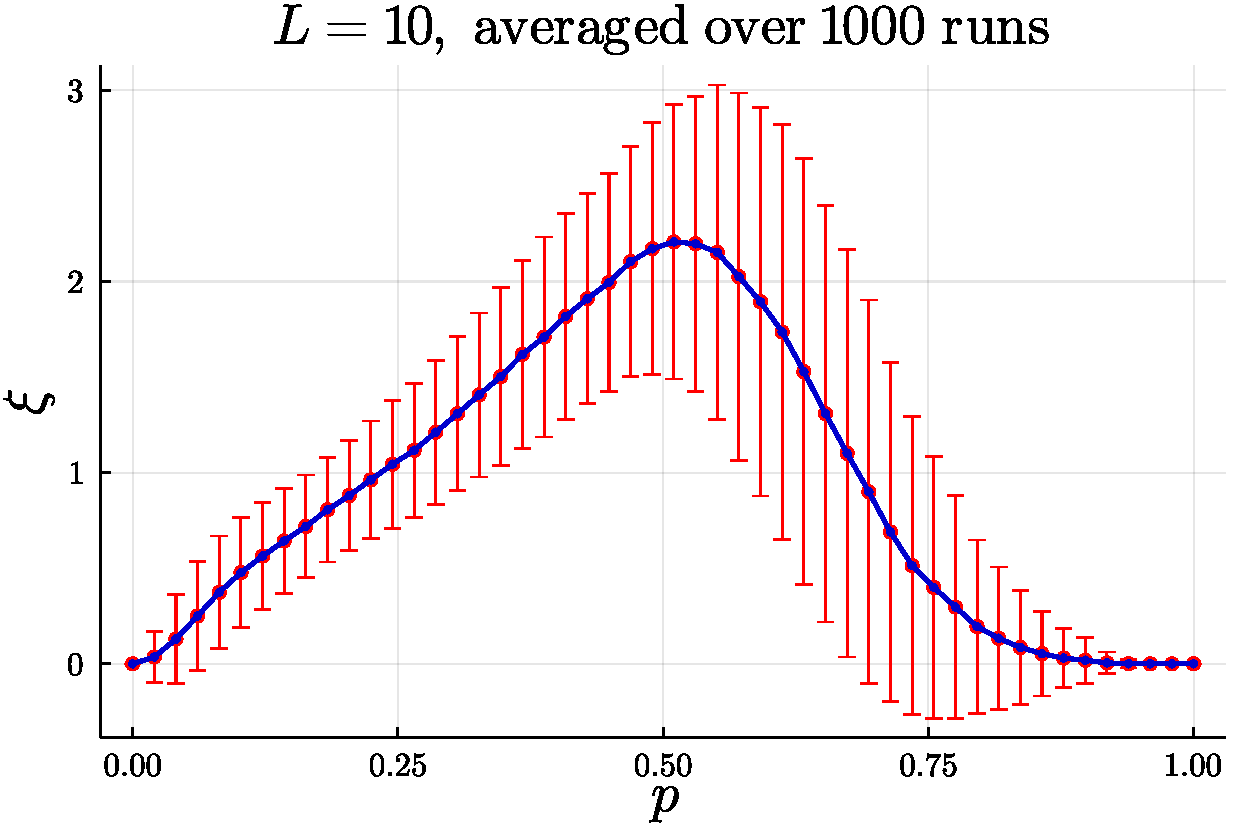
\includegraphics[width=\linewidth]{\percfig/gyration-full-10}
		\end{subfigure}
		\begin{subfigure}{0.45\linewidth}
			\centering
			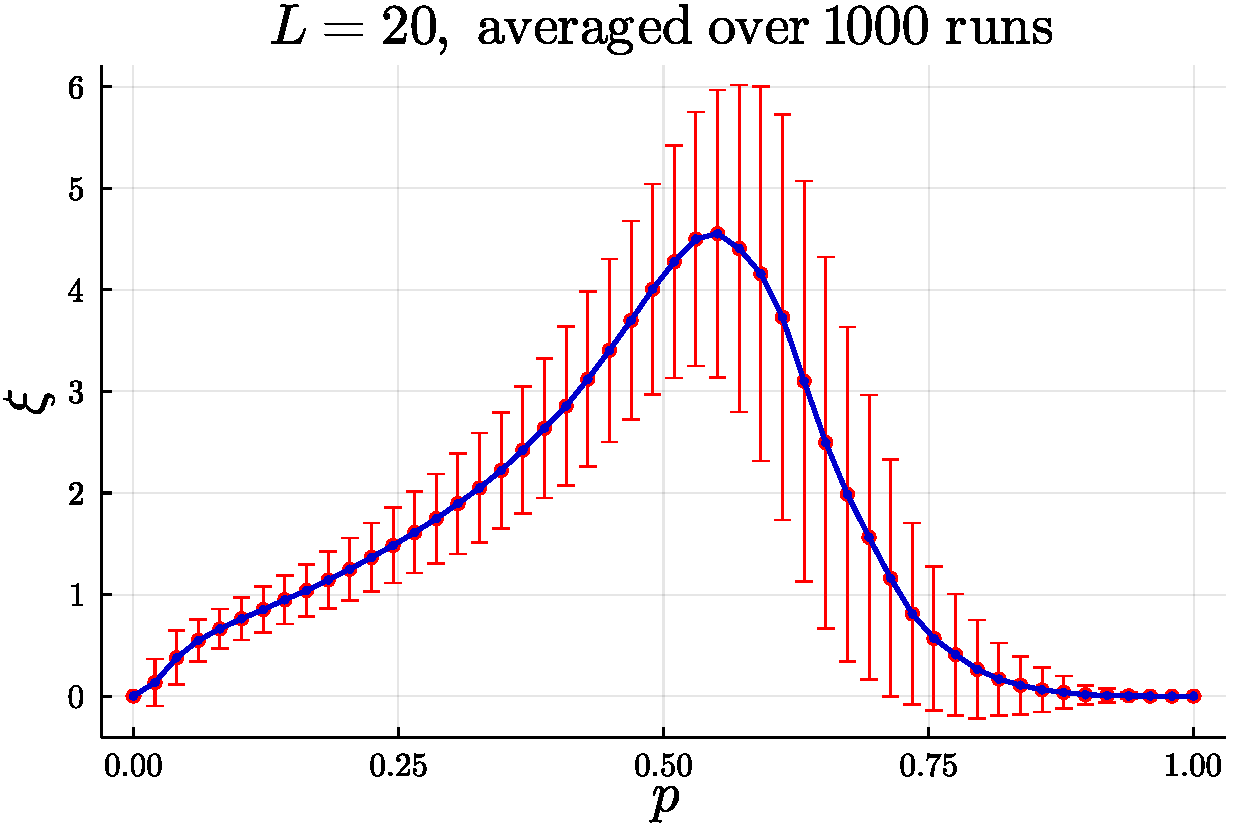
\includegraphics[width=\linewidth]{\percfig/gyration-full-20}
		\end{subfigure}
		\begin{subfigure}{0.45\linewidth}
			\centering
			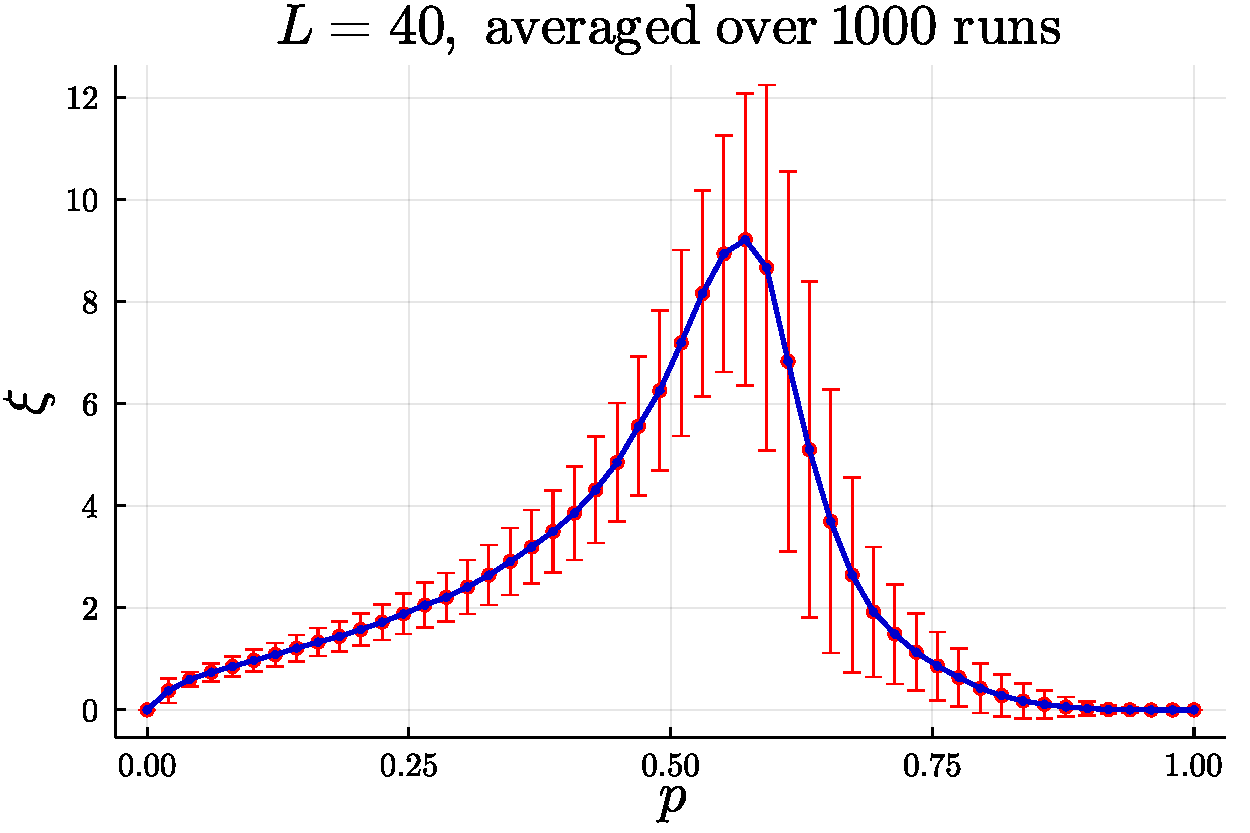
\includegraphics[width=\linewidth]{\percfig/gyration-full-40}
		\end{subfigure}
		\begin{subfigure}{0.45\linewidth}
			\centering
			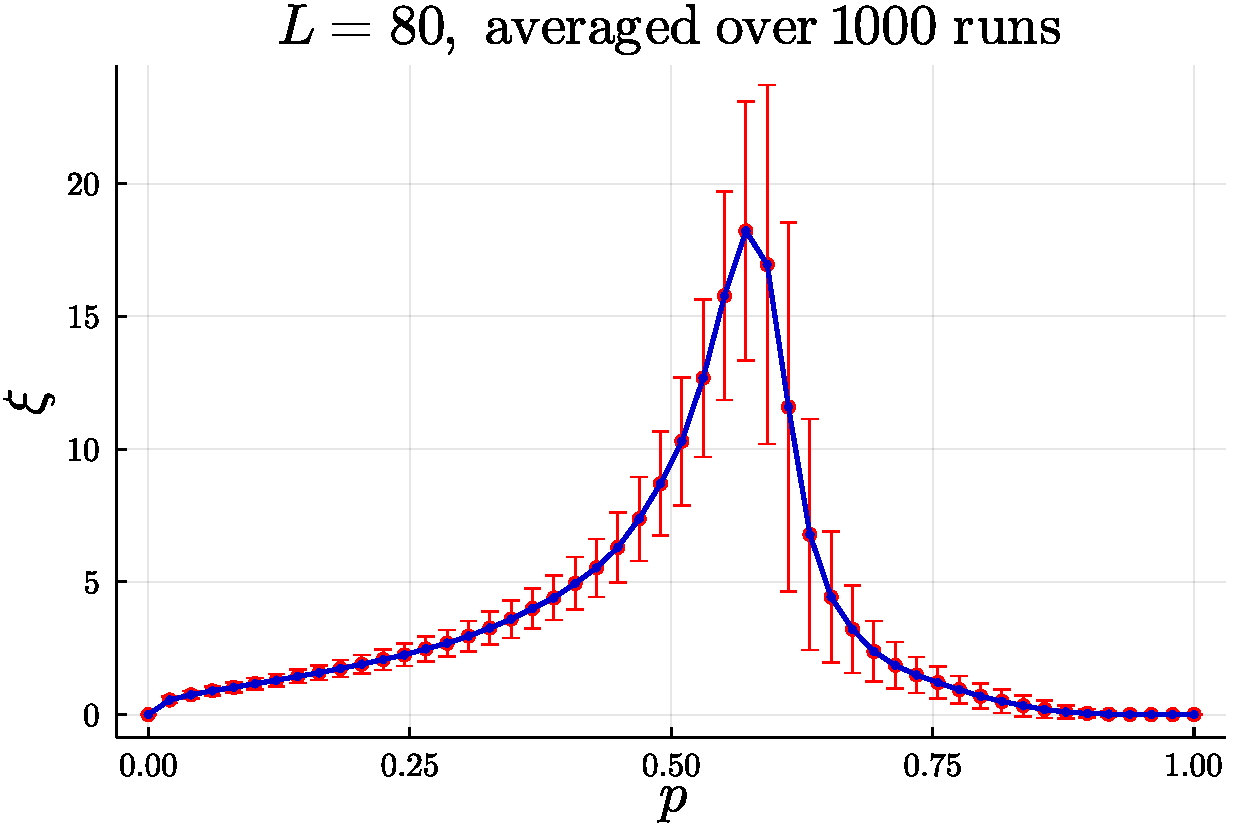
\includegraphics[width=\linewidth]{\percfig/gyration-full-80}
		\end{subfigure}
		\begin{subfigure}{0.45\linewidth}
			\centering
			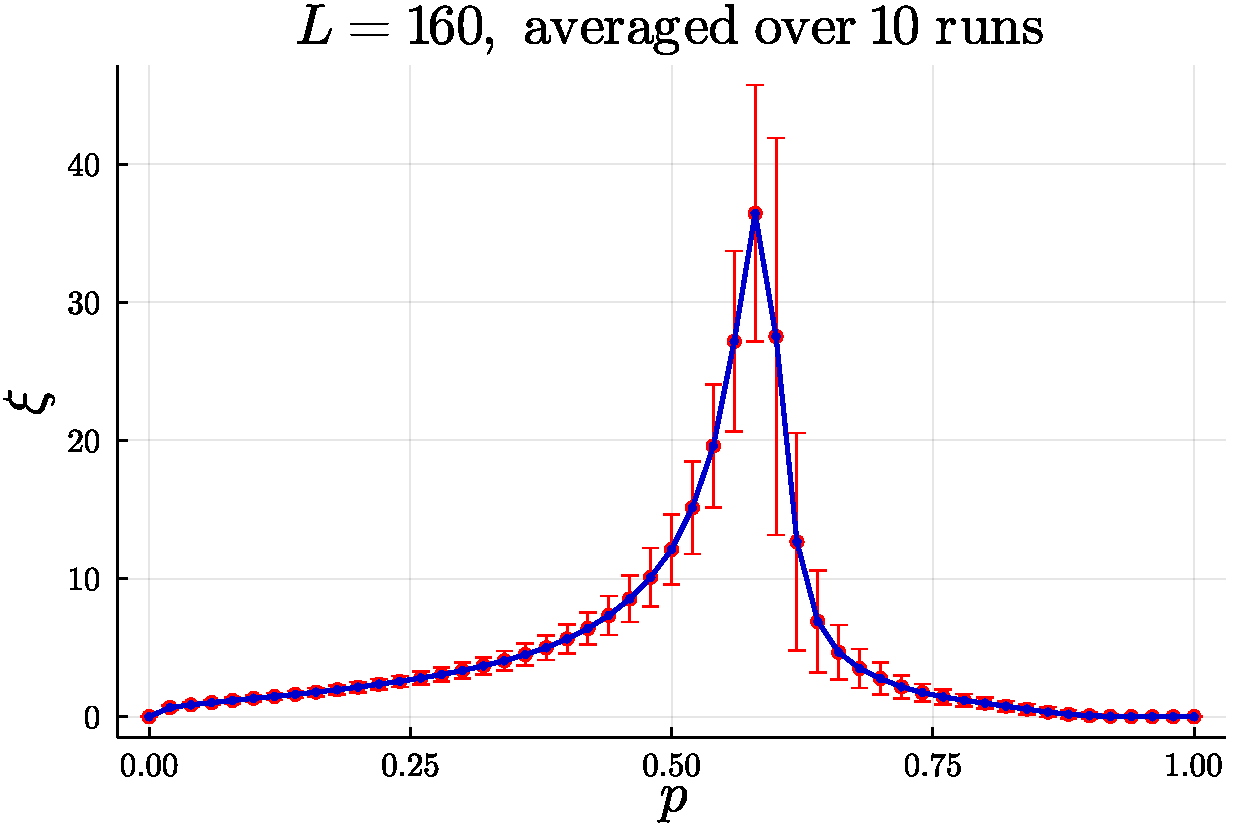
\includegraphics[width=\linewidth]{\percfig/gyration-full-160}
		\end{subfigure}
		\begin{subfigure}{0.45\linewidth}
			\centering
			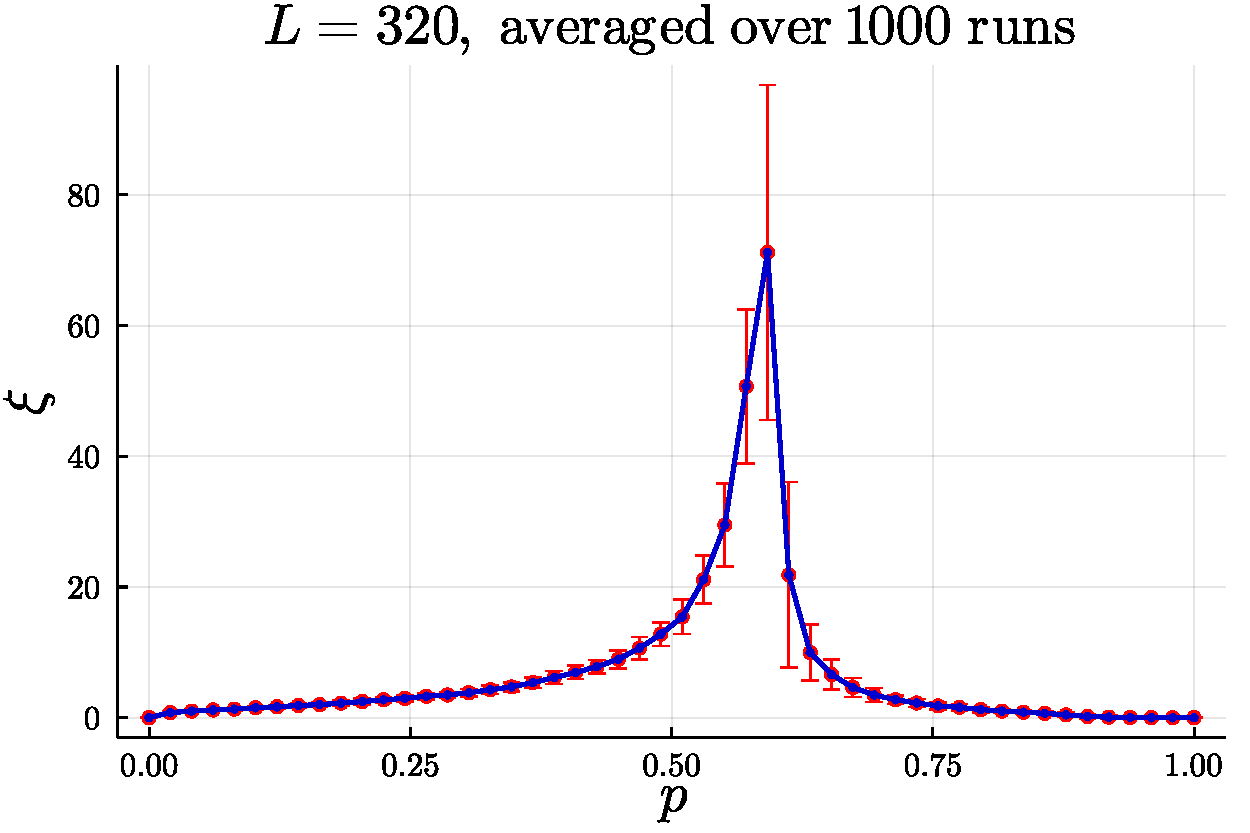
\includegraphics[width=\linewidth]{\percfig/gyration-full-320}
		\end{subfigure}
	\end{figure}
	\newgeometry{top=0.1in, bottom=0.1in, left=0in, right=0in}
	\thispagestyle{empty}
	\begin{figure}
		\centering
		\begin{subfigure}{0.45\linewidth}
			\centering
			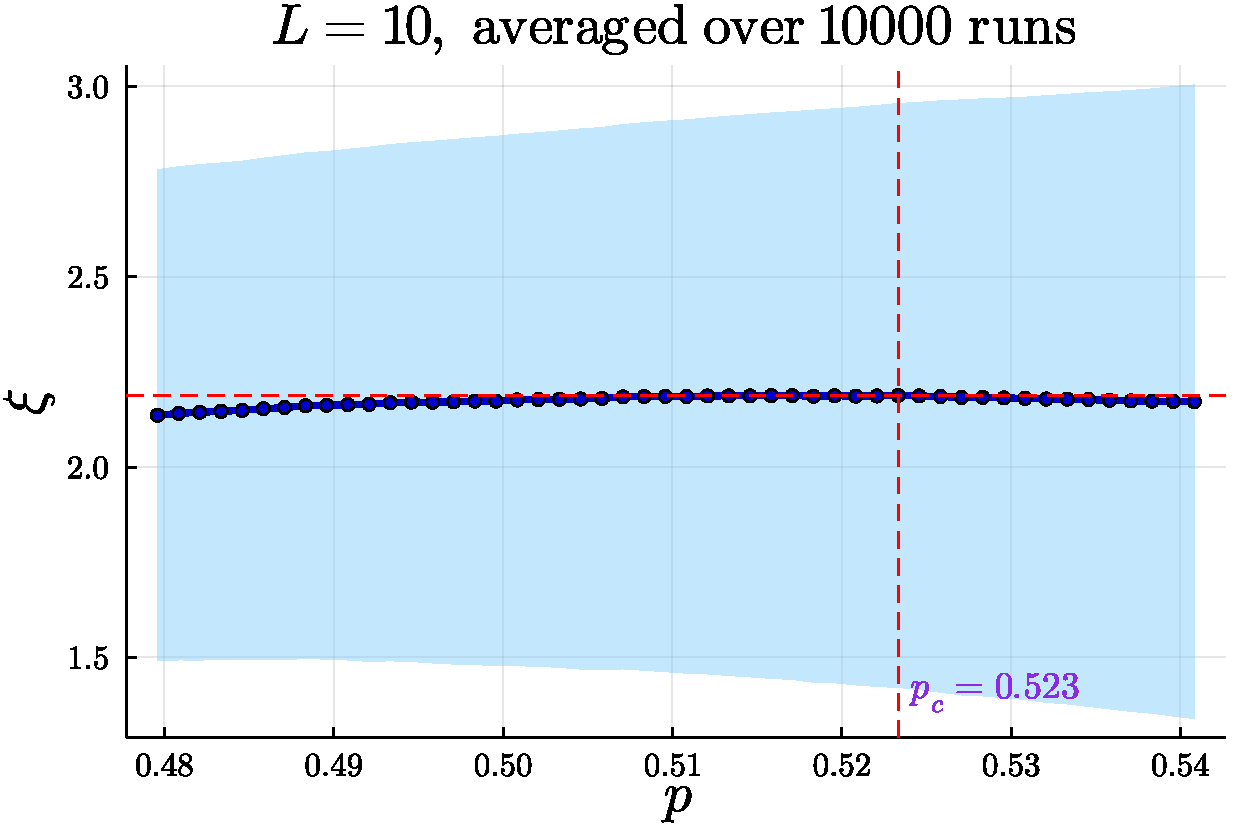
\includegraphics[width=\linewidth]{\percfig/gyration-zoom-10}
		\end{subfigure}
		\begin{subfigure}{0.45\linewidth}
			\centering
			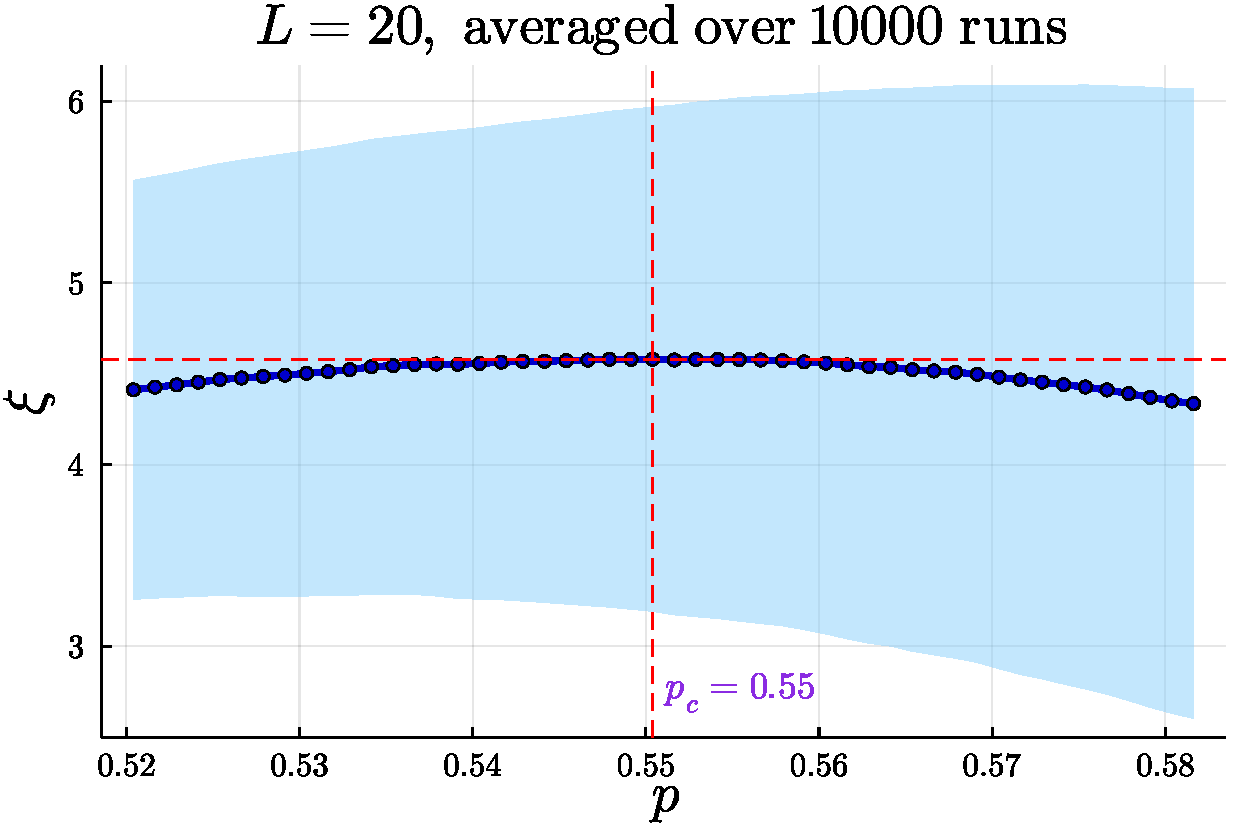
\includegraphics[width=\linewidth]{\percfig/gyration-zoom-20}
		\end{subfigure}
		\begin{subfigure}{0.45\linewidth}
			\centering
			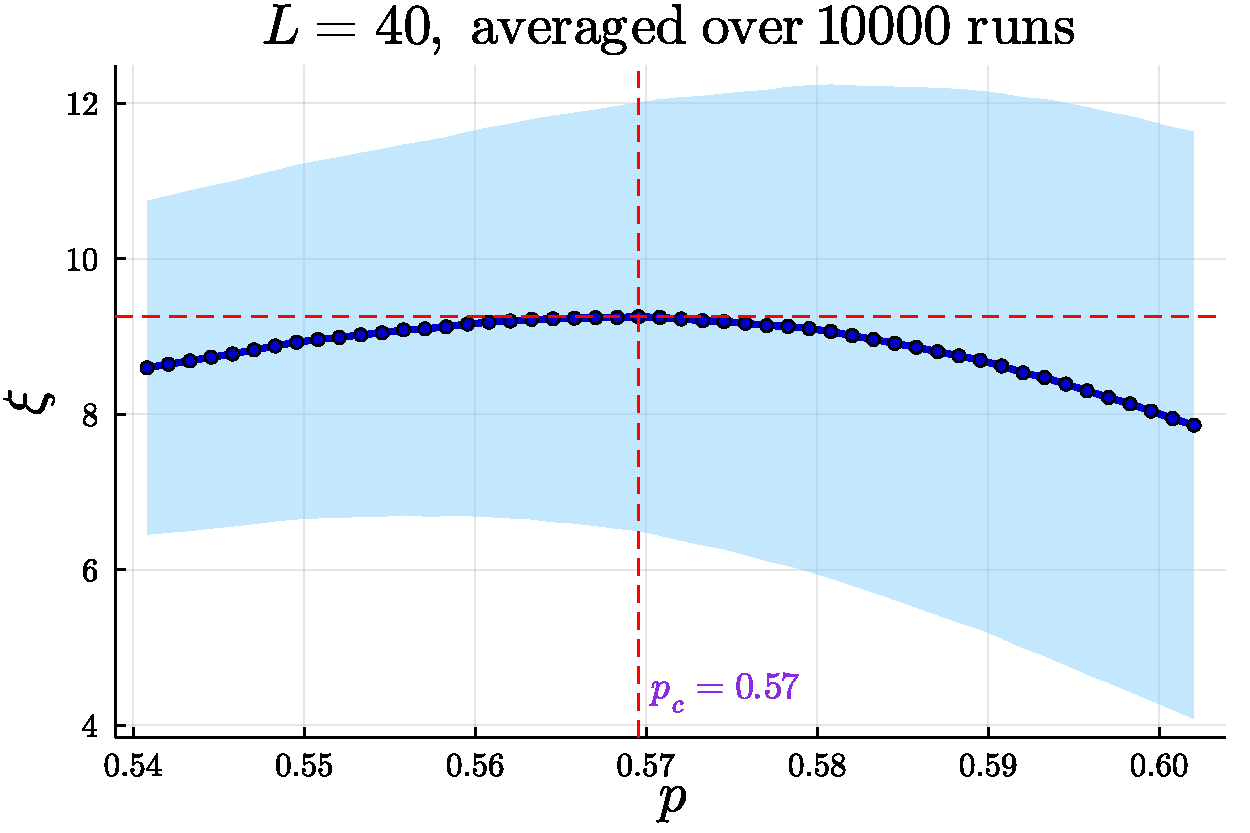
\includegraphics[width=\linewidth]{\percfig/gyration-zoom-40}
		\end{subfigure}
		\begin{subfigure}{0.45\linewidth}
			\centering
			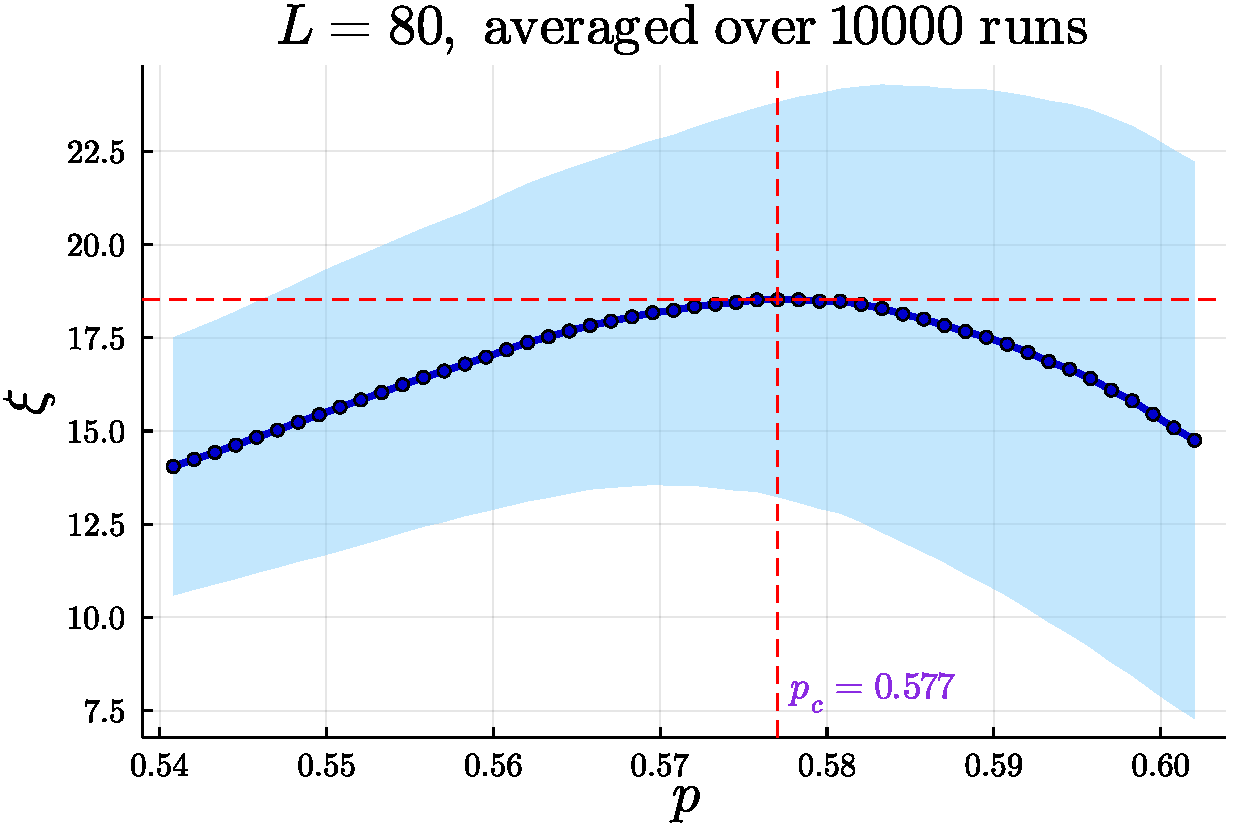
\includegraphics[width=\linewidth]{\percfig/gyration-zoom-80}
		\end{subfigure}
	\end{figure}
	\begin{figure}
		\centering
		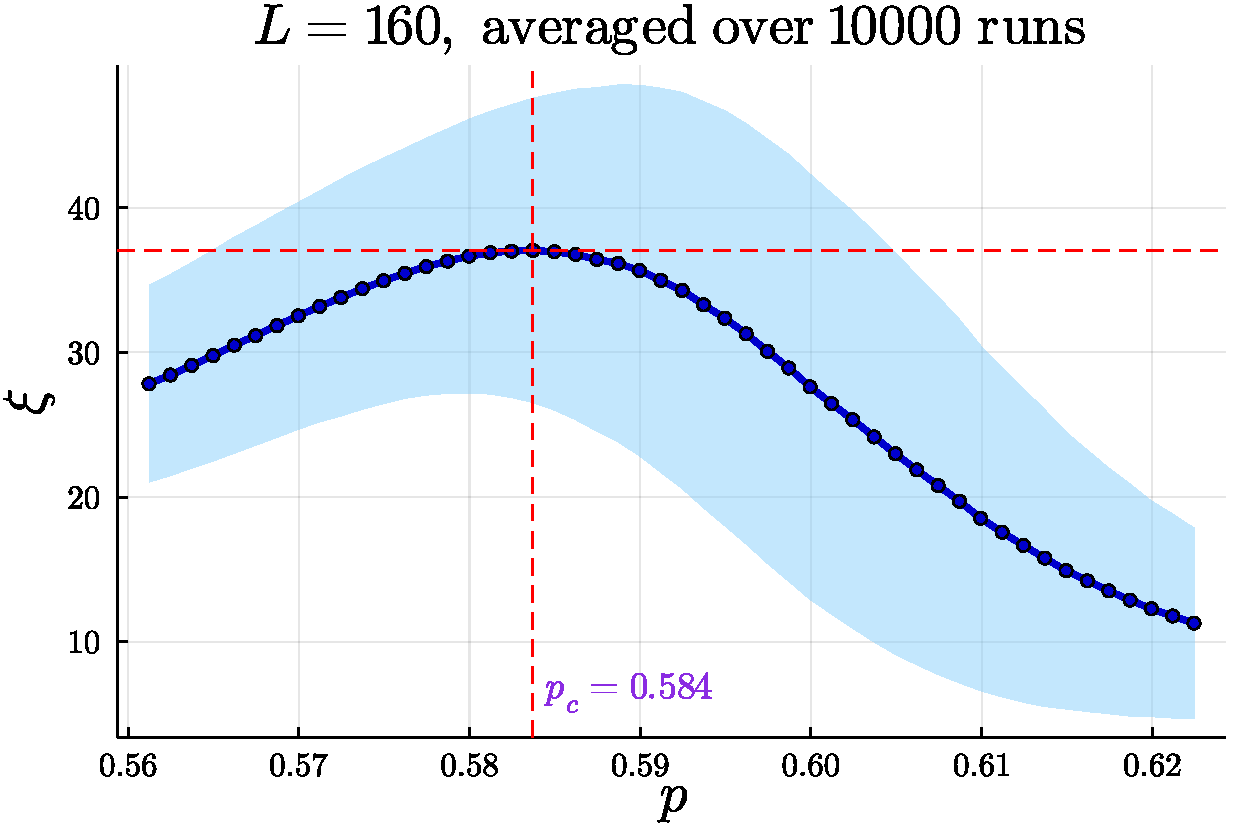
\includegraphics[width=0.9\linewidth]{\percfig/gyration-zoom-160}
	\end{figure}
	\restoregeometry
	\begin{figure}
		\centering
		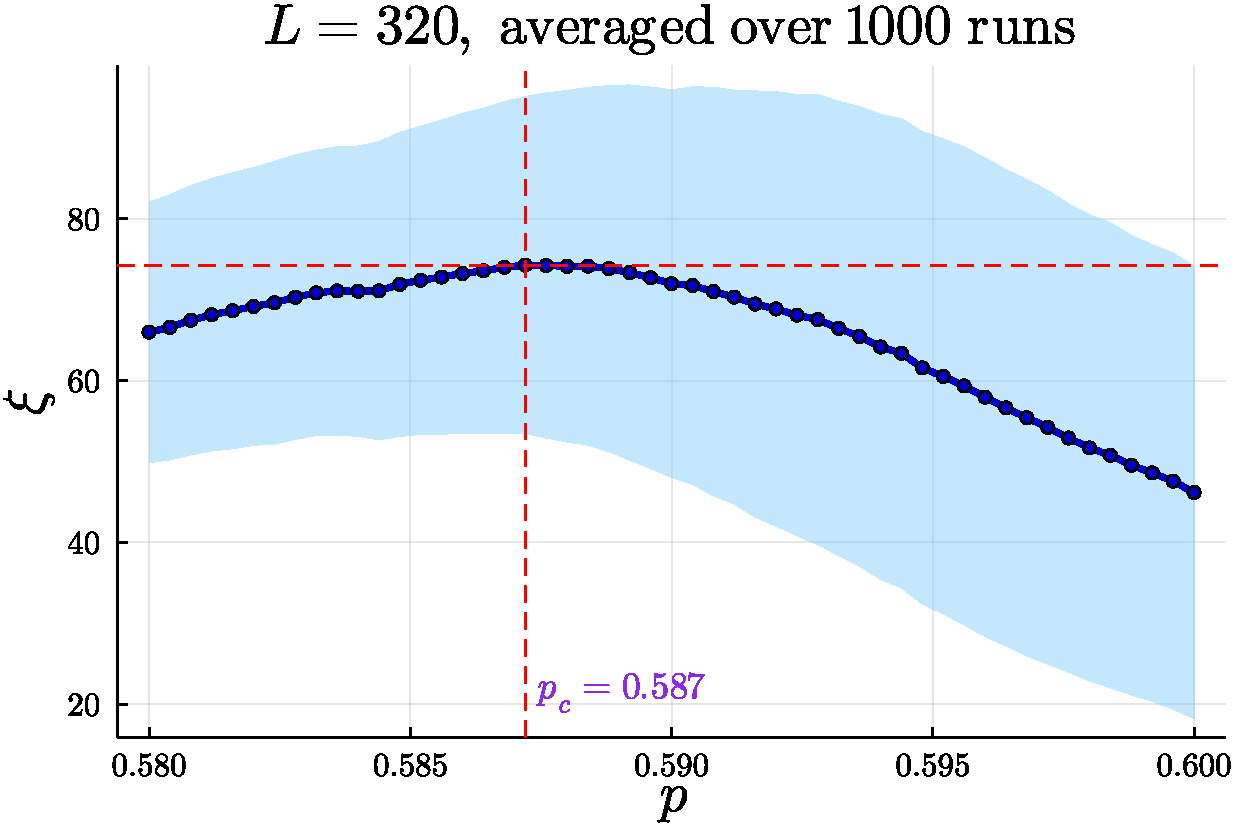
\includegraphics[width=\linewidth]{\percfig/gyration-zoom-320}
	\end{figure}
	Close to the critical probability $p_c$, the following relation holds:
	\begin{equation}
		\xi \sim \abs{p - p_c}^{-\nu}
	\end{equation}
	$\nu$ is called the \emph{critical exponent} for the correlation length $\xi$. In finite lattices, because
	the correlation length is bounded by the lattice length, this relation breaks down at probabilites very
	close to $p_c$. We can find the valuse of $\nu$ with two methods: direct calculation from finite lattices
	or extrapolation.

	In direct calculation, we can use linear regression for the relation
	\begin{equation}
		\log{\xi} = -\nu\log(p - p_c) + C.
	\end{equation}
	This is not especially accurate, because it is based on limited lattices that do not accurately represent unbounded
	trends; The edges of these lattices cut off emerging clusters.
	\begin{figure}
		\centering
		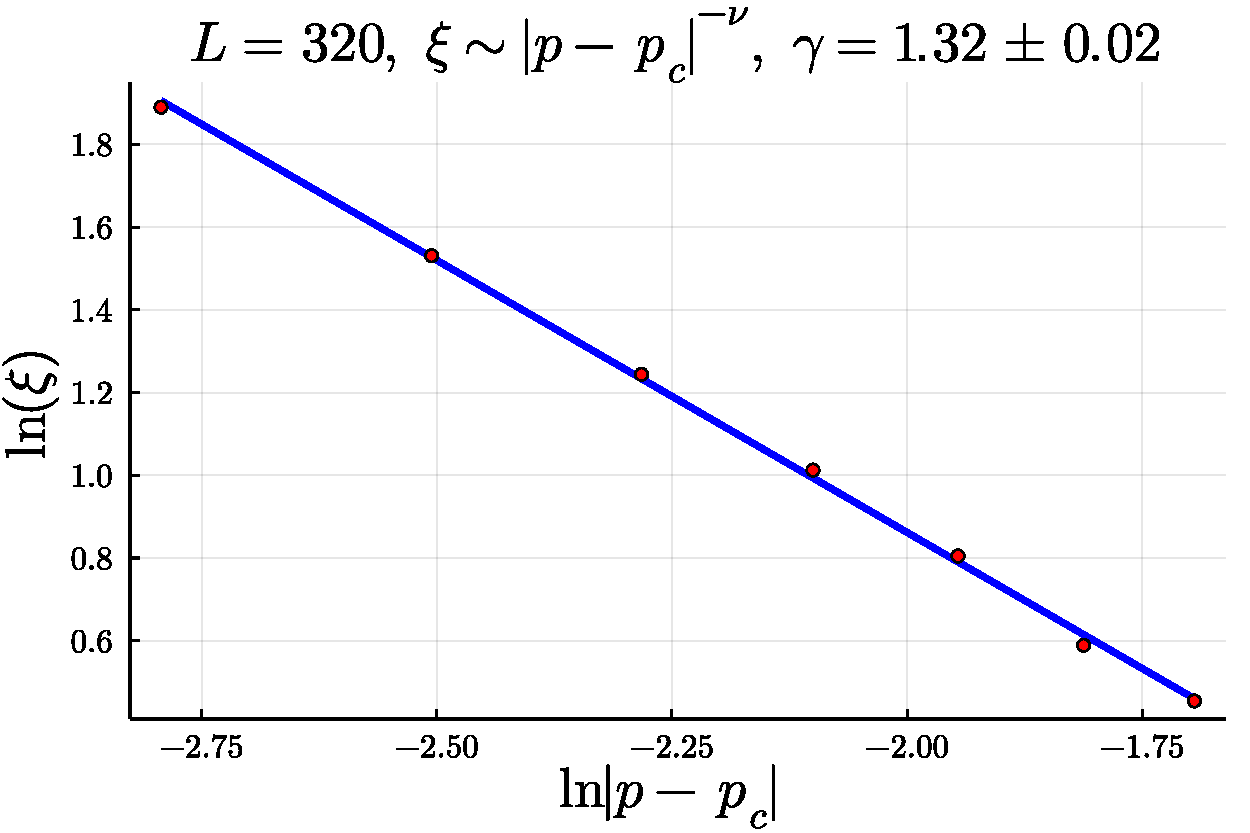
\includegraphics[width=\linewidth]{\percfig/critical-exp}
	\end{figure}

	The extrapolation method is as follows. in finite lattices, the maximum correlation length is proportional to the
	lattice size, since the correlation length at $p_c$ is unbounded for infinite lattices, and is only bounded by the
	edges of the lattice in finite lattices. So, we can approximate the behavior of an infinite lattice by the relation
	\begin{equation}
		\abs{p_c(\infty) - p_c(L)}^{-\nu} = L,
	\end{equation}
	where $p_c(\infty)$ is the infinite lattice's critical probablity and $L$ is the size of a finite lattice.
	Extrapolating $p_c(\infty)$ and $\nu$ with a non-linear curve fit, we get
	\begin{equation}
		p_c(\infty) = 0.5925 ,\qquad \nu = 1.346.
	\end{equation}
	It can be proved that the exact value of $\nu$ is $4/3$ and larges simulations have shown that $p_c(\infty)$ for
	site percolation is $0.5927$, so the accuracy of the extrapolated values are quite good, considering the limited
	sample size.
	
	\subsection{Fractal Dimension}
	The percolation clusters exhibit fractal self-similar behavior. Using a simple breadth-frist search algorithm,
	we can generate clusters in a lattice and calculate their size and radius of gyration to find their
	fractal dimension; If $s$ is the size of the cluster and $d_f$ is the fractal dimension
	\begin{equation}
		s \sim \xi^{d_f},
	\end{equation}
	so, by using linear regression for the relation
	\begin{equation}
		\log{s} = d_f\log{\xi} + C
	\end{equation}
	we can calculate the fractal dimension $d_f$.
	\begin{figure}[htb!]
		\centering
		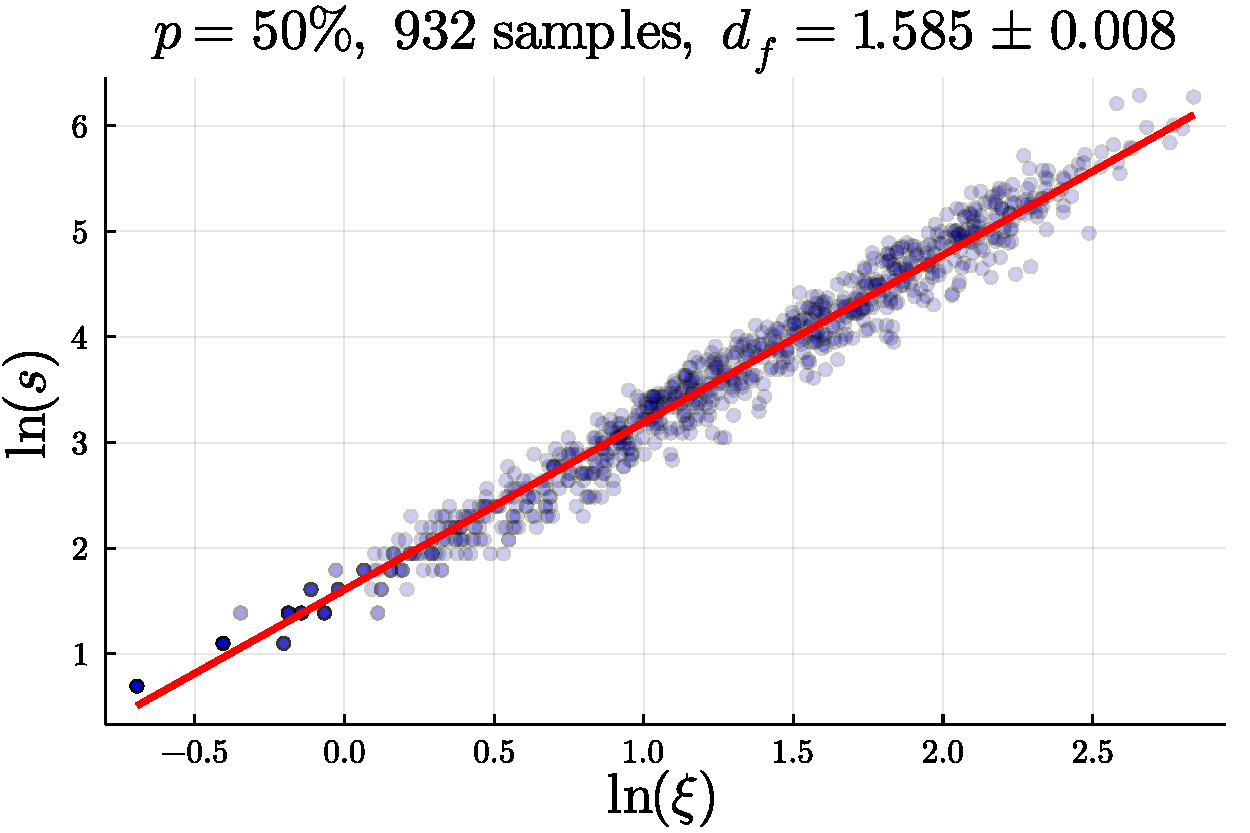
\includegraphics[width=\linewidth]{\percfig/fractal-50}
	\end{figure}
	\begin{figure}[htb!]
		\centering
		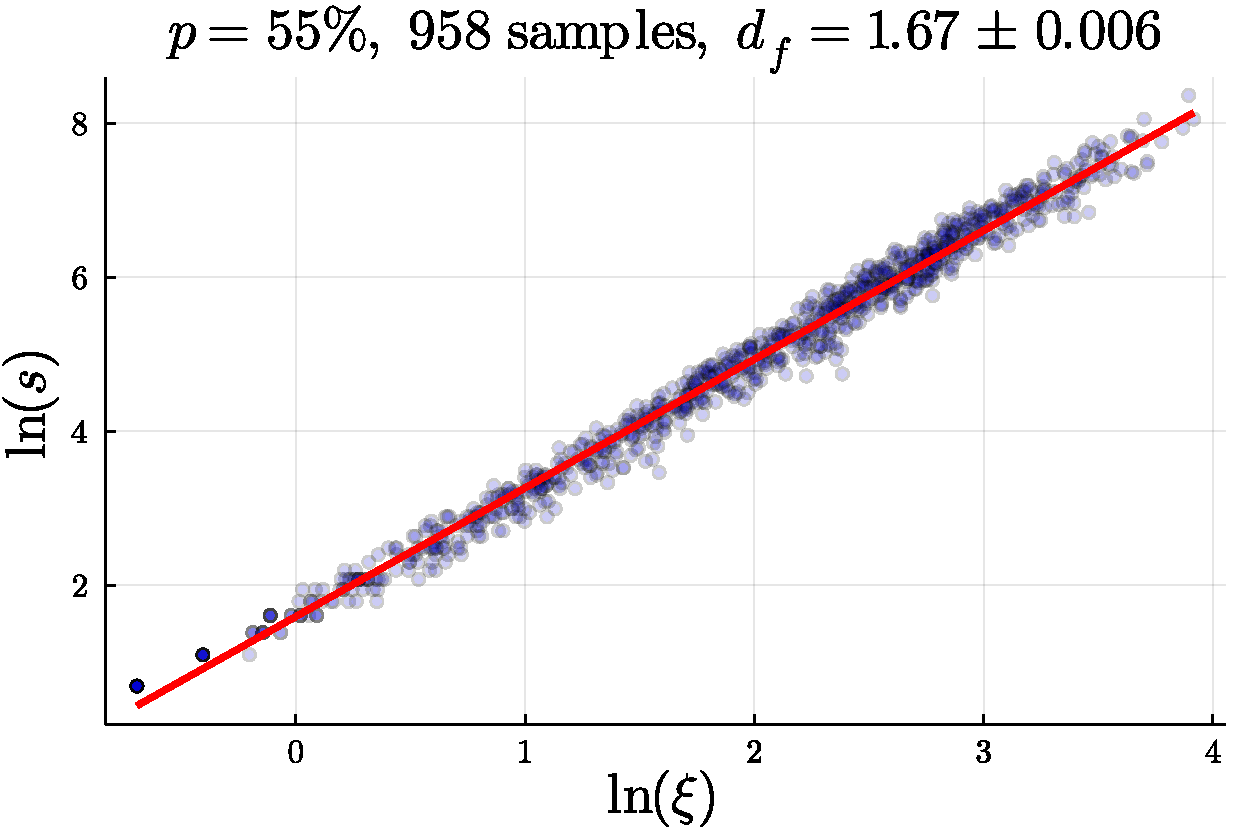
\includegraphics[width=\linewidth]{\percfig/fractal-55}
	\end{figure}
	\begin{figure}[htb!]
		\centering
		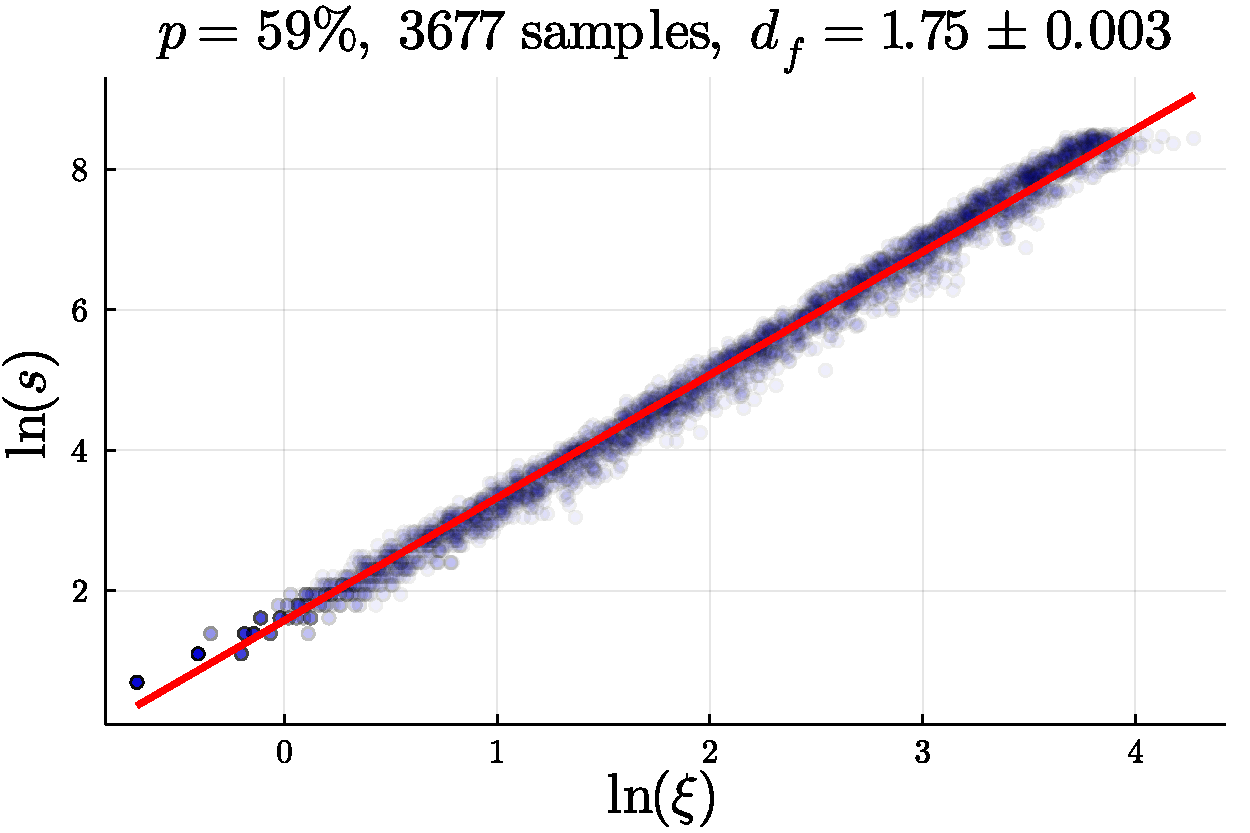
\includegraphics[width=\linewidth]{\percfig/fractal-59}
	\end{figure}
	\section{Random Walk}
	\subsection{Variance}
	We can use the recurrence relation
	\begin{equation}
		x(t) = x(t-\tau) + al,
	\end{equation}
	where $a$ is $+1$ with probability $p$ and $-1$ with probability $q$, to find the variance.
	The calculation is as follows:
	\begin{align}
		\expval{x^2(t)} &= \expval{x^2(t-\tau)} + 2l\expval{ax(t-\tau)} + \expval{a^2}l^2 \\
		&= \expval{x^2(t-\tau)} + l^2 + 2l(p - q)\expval{x(t-\tau)} \\
		&= \expval{x^2(t-\tau)} + l^2 + 2l^2\qty(\frac{t}{\tau}-1)(p - q)^2
	\end{align}
	(Note that $a^2$ is always $1$, and since $a$ is dependant from $x$, $\expval{ax} = \expval{a}\expval{x}$.
	Also, I used $\expval{x(t)} = \frac{l}{\tau}(p-q)t$, which has already been proven in the lecture notes) \\
	Repeating the recurrence relation until it reaches $x(0) = 0$
	\begin{align}
		\expval{x^2(t)} &= \frac{tl^2}{\tau} + \frac{2l^2}{\tau}(p - q)^2 \sum_{n=1}^{t/\tau - 1} n\tau \\
		&= \frac{tl^2}{\tau}\qty[1 + \qty(\frac{t}{\tau} - 1)(p - q)^2].
	\end{align}
	Substituting into the variance,
	\begin{align}
		\sigma^2(t) &= \expval{x^2(t)} - \expval{x(t)}^2 \\
		&= \frac{tl^2}{\tau}\qty[1 + \qty(\frac{t}{\tau} - 1)(p - q)^2] - \frac{t^2l^2}{\tau^2}(p-q)^2 \\
		&= \frac{tl^2}{\tau}\qty[1 - (p - q)^2].
	\end{align}
	But
	\begin{equation}
		p+q = 1 \implies (p+q)^2 = 1 \implies p^2 + q^2 = 1 - 2pq,
	\end{equation}
	and using this to simplify the expression
	\begin{equation}
		\sigma^2(t) = \frac{tl^2}{\tau}\qty[1 - (p^2 + q^2) + 2pq] = \frac{tl^2}{\tau}\qty[1 - 1 + 2pq + 2pq]
	\end{equation}
	\begin{empheq}[box=\fbox]{equation}
		\sigma^2(t) = \frac{4l^2}{\tau}pqt
	\end{empheq}
	\subsection{Simulation}
	\begin{figure}
		\centering
		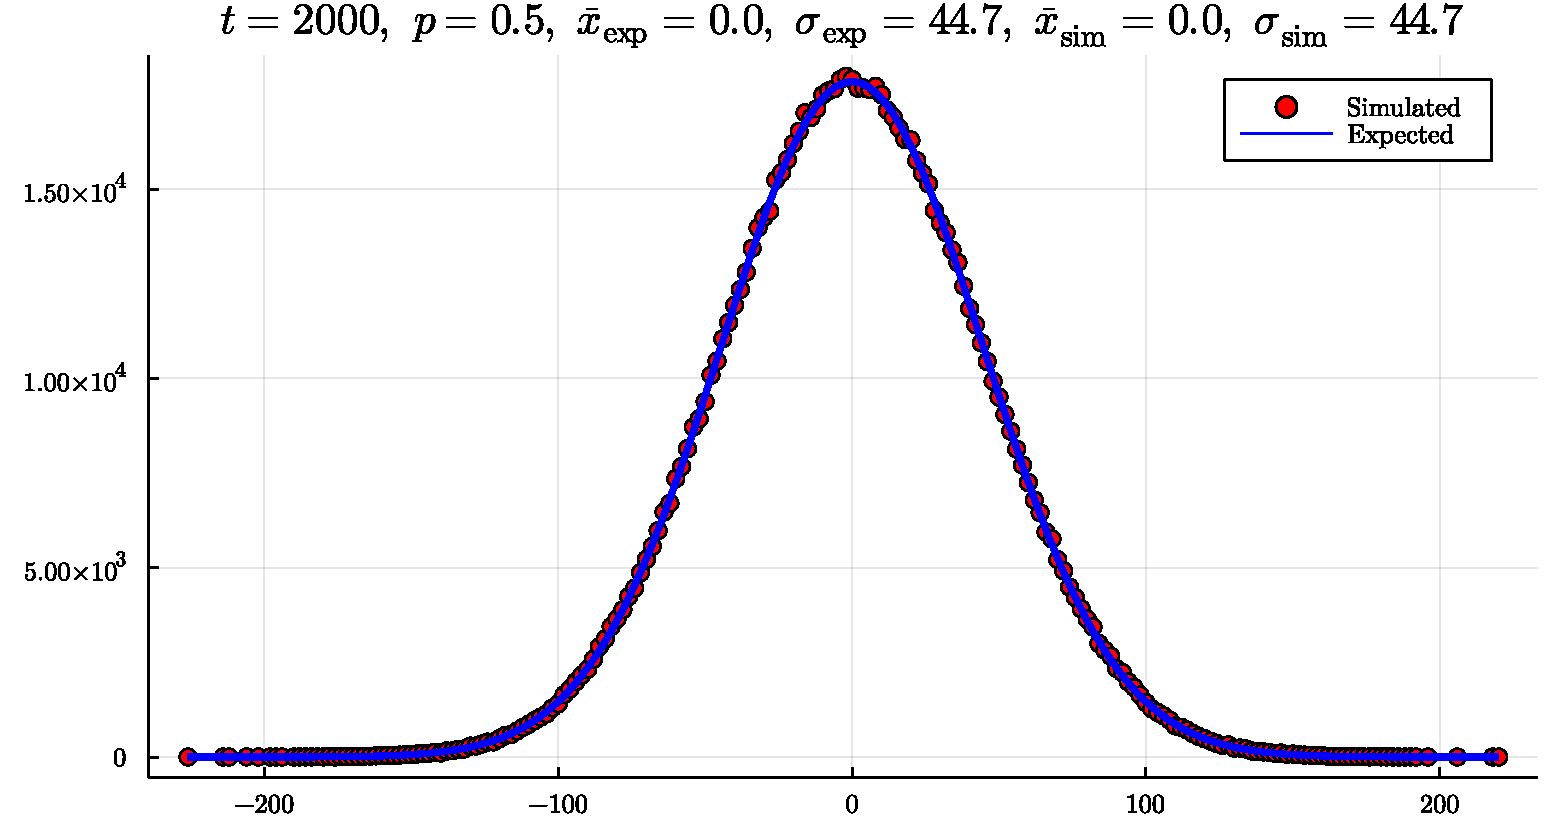
\includegraphics[width=\linewidth]{\rwfig/randomwalk-50}
	\end{figure}
	\begin{figure}
		\centering
		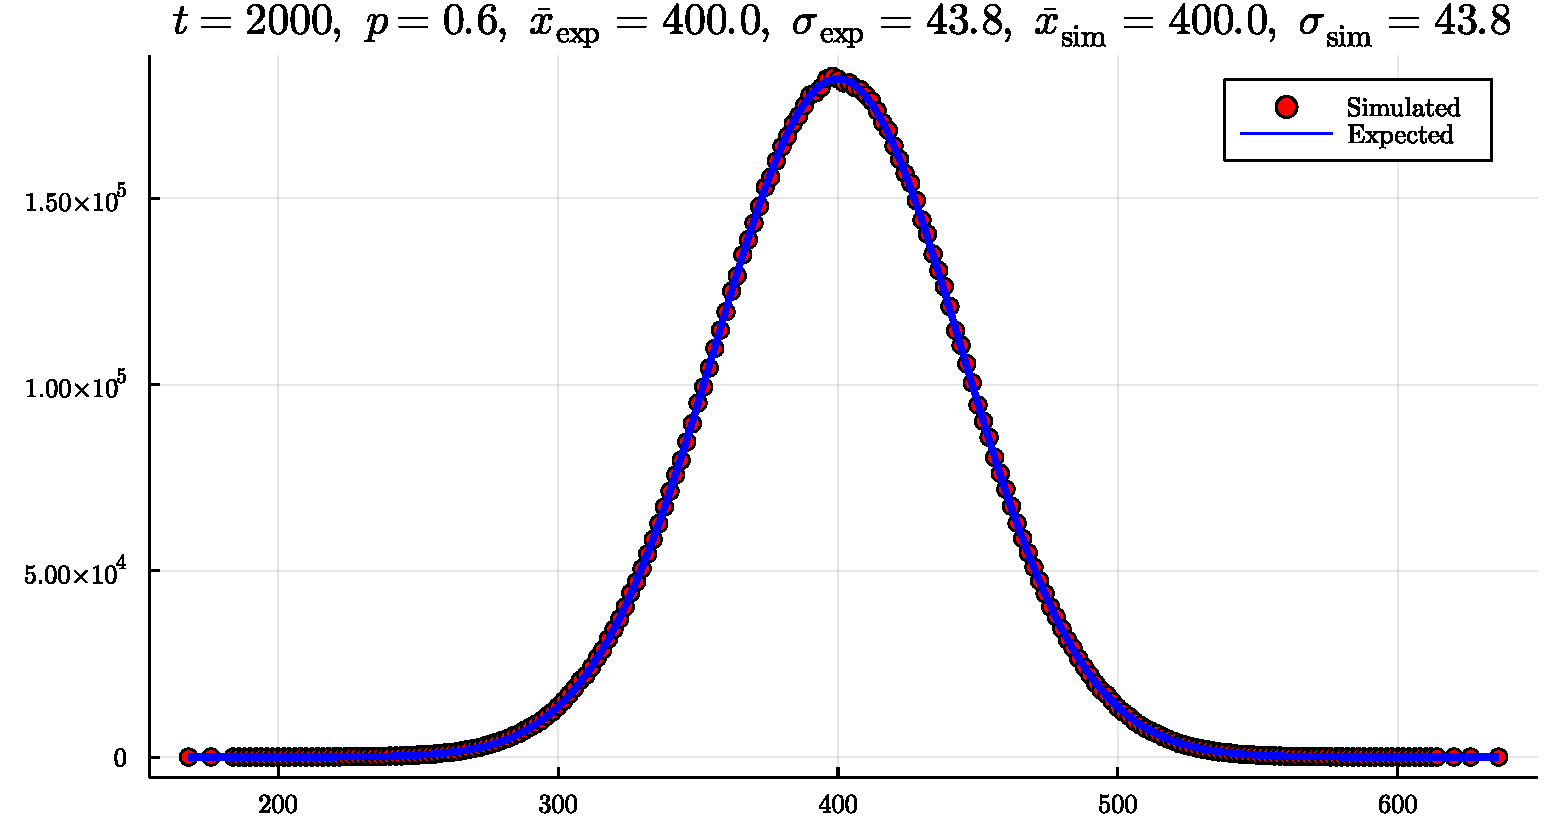
\includegraphics[width=\linewidth]{\rwfig/randomwalk-60}
	\end{figure}
	\begin{figure}
		\centering
		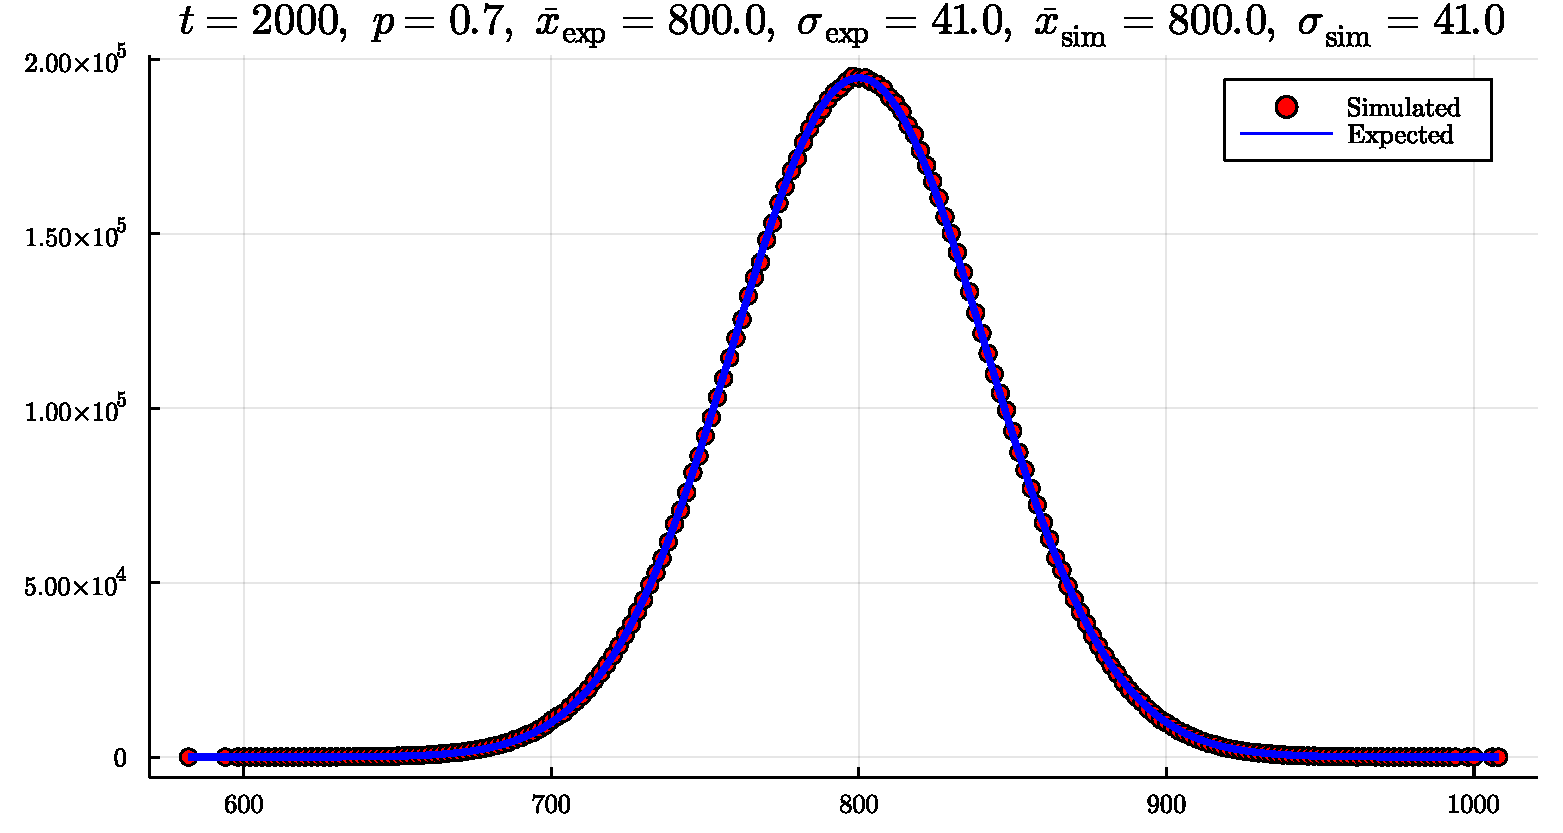
\includegraphics[width=\linewidth]{\rwfig/randomwalk-70}
	\end{figure}
	\begin{figure}
		\centering
		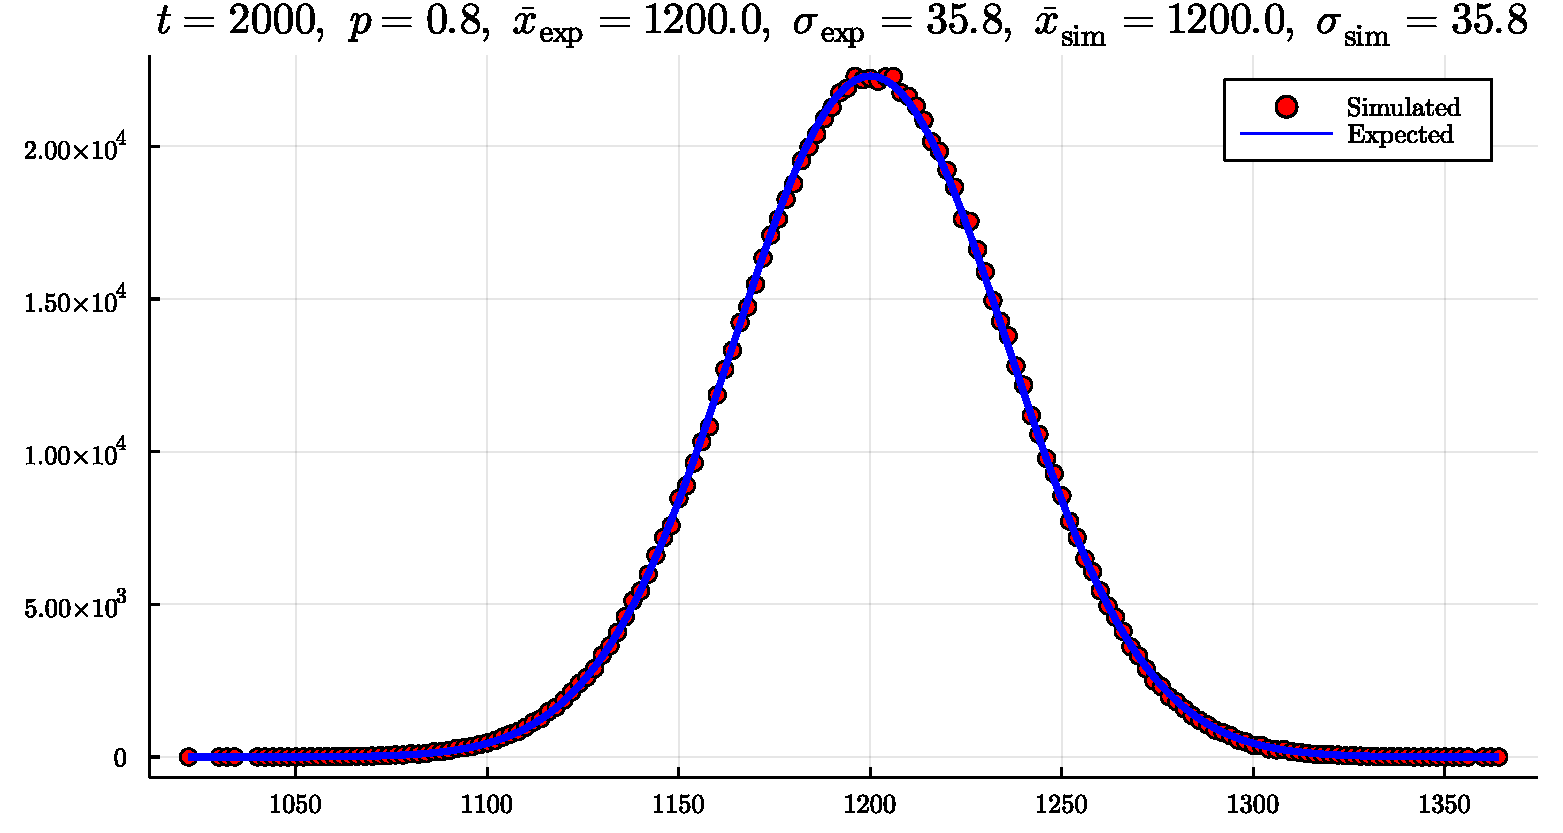
\includegraphics[width=\linewidth]{\rwfig/randomwalk-80}
	\end{figure}
\end{document}
